\section{Master's Project: Implementation}

\subsection{MOSIS Packages Supported}
In our senior project, we were able to support 11x11, 12x12, and 13x13 MOSIS packages. Because we need more FPGA pins to configure external hardware in this project, we are only able to support 11x11 and 12x12 packages on our DUT Board's 13x13 ZIF socket. See Figure \ref{fig:mosis_packages_supported} for details.

\begin{figure}
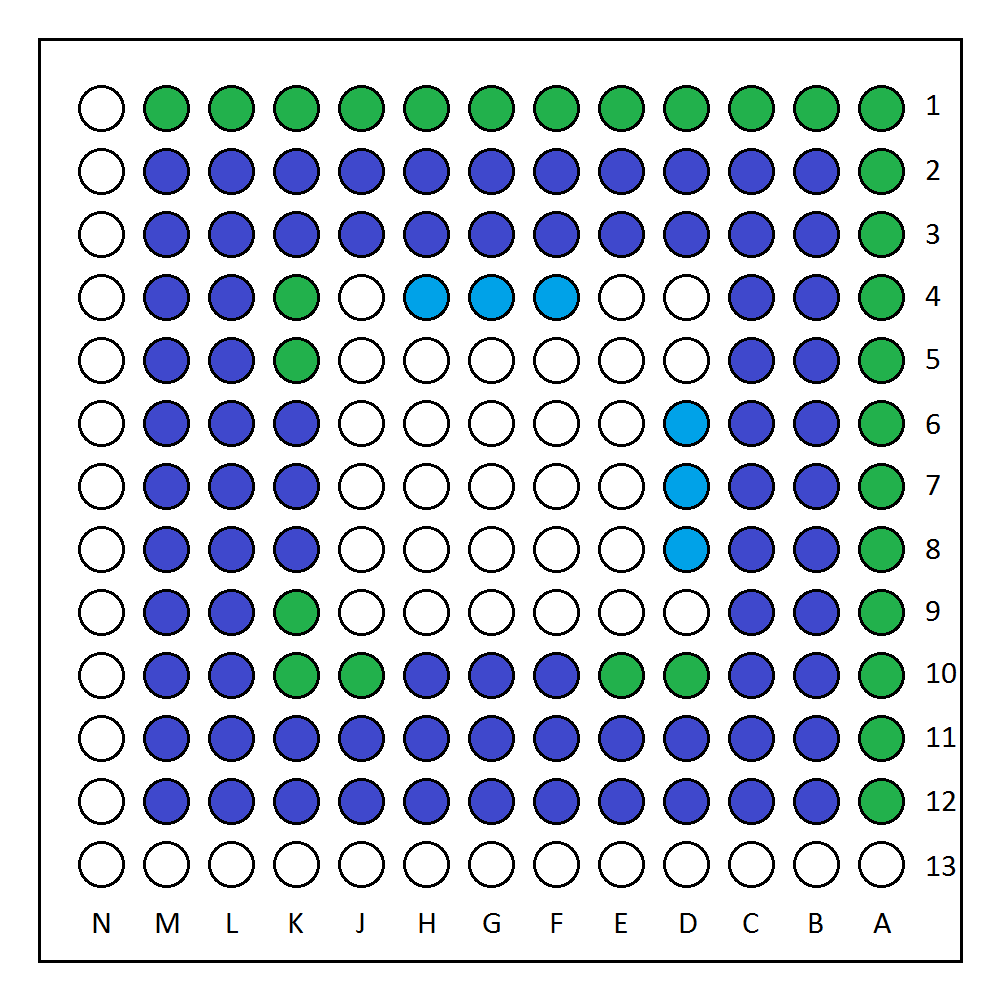
\includegraphics[width=1.0\textwidth]{mosis_packages_supported.png}
\caption{MOSIS packages supported by our tester. Blue: Pins for 11x11 packages. Green: Pins for 12x12 packages. Purple: Pins shared by 11x11 and 12x12 packages.}
\label{fig:mosis_packages_supported}
\end{figure}

\subsection{BeagleBone Black Web Server and C Code}
TODO: Norm (web server code), Daniel (C code)
\subsection{Verilog for Numato Saturn}
For a detailed understanding of the Verilog coded onto the Numato Saturn, we advise readers to study to the well-commented Verilog code on our repository. In this section, we provide a synopsis of the Verilog design.

Our Verilog design consists of one "central" finite state machine (FSM) that communicates with controllers for the following components: 
\begin{itemize}
	\item Block RAM.
	\item Counters.
	\item DUT input/output signals.
	\item Output buffers.
	\item SRAM blocks.
	\item UART.
	\item Voltage translators.
\end{itemize}

We first describe how the BeagleBone Black communicates with the FPGA. Then, we further detail each controller and finally the central FSM logic.

\subsubsection{BeagleBone Black - FPGA Communication Protocol}
The BeagleBone Black serves as a master device, the FPGA a slave device. The two boards communicate with each other via UART (baud rate 115200, one start bit, eight bits per word, one stop bit, no parity bit). 16 bytes are always sent at a time between the two devices.

The BeagleBone Black may send the following commands (note that only the least significant byte in the transfer is recognized): 
\begin{itemize}
\item 8'b00000000: The next 16 bytes are a template vector.
\item 8'b00000001: The next 16 bytes are a force-format vector.
\item 8'b00000010: The next 16 bytes are a cycle vector.
\item 8'b00000011: The next 16 bytes are an input vector.
\item 8'b00000100: The next 16 bytes will contain, starting with the least significant byte and one byte per entity, DELAY 1, DELAY 2, WIDTH, LENGTH.
\item 8'b00000101: The FPGA should execute all input vectors.
\item 8'b00000110: After the FPGA executes all tests, the counters are reset. The FPGA should send back the SRAM contents at the address, then increment the counter. Note that the BeagleBone Black must invoke this command as many times as there are input vectors.
\end{itemize}

The FPGA may send the following commands: 
\begin{itemize}
\item 8'b00000000: Acknowledge of command received from BeagleBone Black.
\item 8'b00000001: This command is sent if the BeagleBone Black requests that all input vectors be executed, but no input vectors have been loaded.
\item 8'b11111111: Unknown command received.
\end{itemize}

Figure \ref{fig:uart_vector_transfer} details  how a template, force-format, cycle, or input vector is sent to the FPGA. 126 bits consist of the vector data while the uppermost two bits (T1 and T0) indicate which template the vector is associated with. Thus, up to four template vectors are allowed.

\begin{figure}
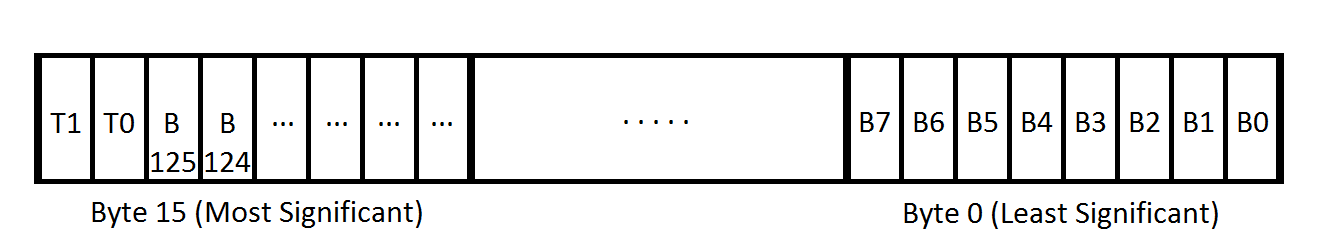
\includegraphics[width=1.0\textwidth]{uart_vector_transfer.png}
\caption{UART bit-vector transfers.}
\label{fig:uart_vector_transfer}
\end{figure}

\subsubsection{Block RAM Controller}
The block RAM on the Spartan-6 FPGA is configured to support 13-bit addresses, 32-bit reads/writes, and dual-port access. Block RAM is partitioned into four sections, as shown in Figure \ref{fig:block_ram_layout}. Note that all bit vectors are 128 bits in length, so any read/write requires two accesses (using two ports allows for 64-bit reads/writes per clock cycle).

With 32 kilobits of block RAM available, the FPGA can store 256 vectors. Up to four template vectors, and thus four FF and cycle vectors, are supported, allowing for a total of 244 input vectors to be stored.

The controller abstracts this partitioning of block RAM, enabling users to read/write a specified type of vector. The controller also keeps track of how many input vectors have been read/written during test execution.

\begin{figure}
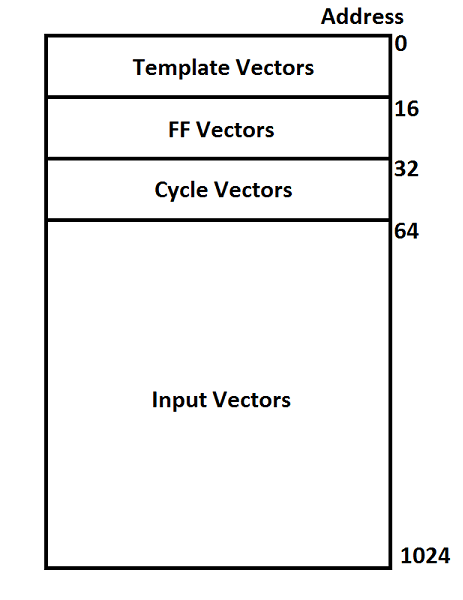
\includegraphics[width=1.0\textwidth]{block_ram.png}
\caption{Block RAM layout.}
\label{fig:block_ram_layout}
\end{figure}

\subsubsection{Counter Controller}
This controller allows a user to advance or reset the counter.

\subsubsection{DUT Controller}
This controller consists of double-buffered registers for test-cycle logic. Figure \ref{fig:block_ram_layout} illustrates our symbol for a double-buffered register, and Figure \ref{fig:test_cycle_logic} illustrates the logic per input vector bit.

The idea is as follows: an input vector bit (SIG), along with the associated FF bit, CYCLE bit, and TEMPLATE bit are loaded into double-buffered registers. 
\begin{itemize}
\item The FF bit denotes whether SIG should follow R0 or DRNZ L logic.
\item The CYCLE bit denotes whether SIG should force its value on the DELAY 1 or DELAY 2 edge. 
\item The TEMPLATE bit denotes whether SIG maps to an input on the DUT (in which case the tristate buffer is enabled) or an output of the DUT (in which case the tristate buffer is disabled).
\end{itemize}

Once all of the appropriate signals have been loaded into the double-buffered registers, they may be transferred at the beginning of a test cycle. Note that separate load and transfer signals are associated with each double-buffered register (not shown in Figure \ref{fig:test_cycle_logic}). 

\subsubsection{Output Buffer Controller}
This controller provides two commands: load the output buffers (parallel-to-serial shift registers) with whatever signals lie on the inputs, and clock the contents of the output buffers into the FPGA. Note that because the shift-registers are daisy-chained on the DUT Board, we deliberately picked very slow registers. As such, the controller carefully accounts for the propagation delay of the chips.

\subsubsection{SRAM Controller}
This controller allows a user to configure the CS, OE, and WE lines on the DUT Board's SRAM blocks.

\subsubsection{UART Controller}
This controller notifies when data has been retrieved over UART and allows users to abstractly transmit data over UART. Note that data read/written is always 16 bytes (128 bits).

\subsection{Central FSM}
With nearly 60 states, explaining the operation of this FSM through a state-flow diagram is intractable. Again, users seeking more information should study the Verilog code itself. We summarize the FSM's operation as follows: 
\begin{enumerate}
\item Remain IDLE until UART data is received.
\item Decode the UART command.
\item If we are told to expect a template/force-format/cycle/input vector: 
  \begin{enumerate}[label=\arabic*.]
    \item Transmit an acknowledgement.
    \item Wait for the vector to arrive.
    \item Store the vector in block RAM.
    \item Transmit an acknowledgement.
    \item Return to IDLE.
  \end{enumerate}
\item Else, if we are told to expect test cycle configuration data: 
  \begin{enumerate}[label=\arabic*.]
    \item Transmit an acknowledgement.
    \item Wait for the vector to arrive.
    \item Store the DELAY 1, DELAY 2, WIDTH, and LENGTH data into designated registers.
    \item Transmit an acknowledgement.
    \item Return to IDLE.
  \end{enumerate}
\item Else, if we are told to execute tests: 
  \begin{enumerate}[label=\arabic*.]
  	\item If no input vectors exist, transmit an error and return to IDLE.
    \item Load the first input vector from block RAM into the corresponding double-buffered register.
    \item Using the upper two bits of the input vector, load the corresponding template, force-format, and cycle vectors into the corresponding double-buffered registers.
    \item  Transfer all of the double-buffered registers' contents, then load the test cycle. 
    \item Fetch the next input vector from block RAM. 
    \item If the template bits of the new input vector are the same, load the input vector bits and transfer them at the end of the test cycle.
    \item Else, pause real-time testing, fetch the corresponding template, force-format, and cycle vectors from block RAM into the corresponding double-buffered registers.
    \ Transfer the new vector bits and resume testing.
    \item If more input vectors exist, go to step 2.
    \item Else, transmit an acknowledgement.
    \item Return to IDLE.
  \end{enumerate}
\item Else, if we are told to transmit SRAM data: 
  \begin{enumerate}[label=\arabic*.]
    \item Load the SRAM data into the output buffers.
    \item Clock in the SRAM data from the output buffers.
    \item Transmit the data back to the BeagleBone Black.
    \item Return to IDLE.
  \end{enumerate}
  \item Else, transmit an error code and return to IDLE.
\end{enumerate}

Regarding hardware signals: 
\begin{itemize}
	\item SRAM should be enabled in \textit{write-mode} at the beginning of a test cycle and disabled at the trailing edge of a test cycle.
	\item SRAM should be enabled in \textit{read-mode} when reading data into the output buffers.
	\item After a test cycle, counters should be incremented. After all test cycles are executed, counters should be reset.
	\item Voltage translators are always enabled except when reading from SRAM.
	\item Output buffers are disabled except when reading from SRAM.
\end{itemize}

\begin{figure}
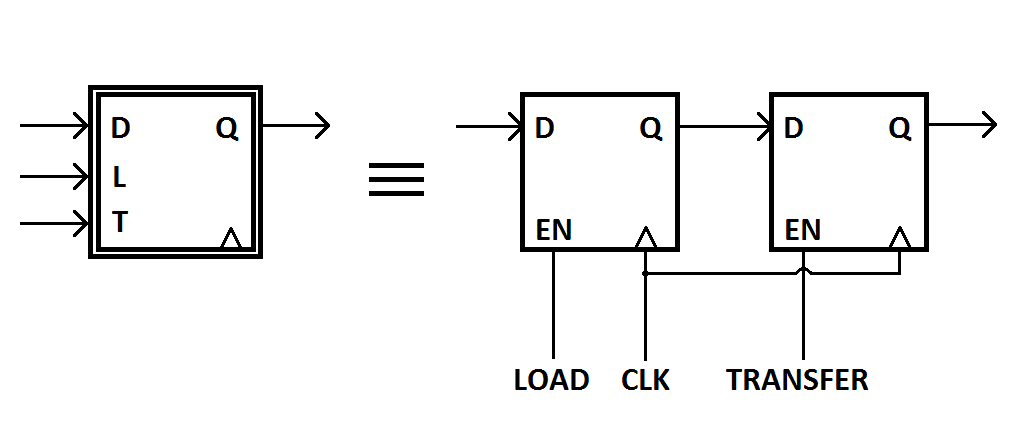
\includegraphics[width=1.0\textwidth]{double_buffered_reg.png}
\caption{Double-buffered register symbol.}
\label{fig:double_buf_reg}
\end{figure}

\begin{figure}
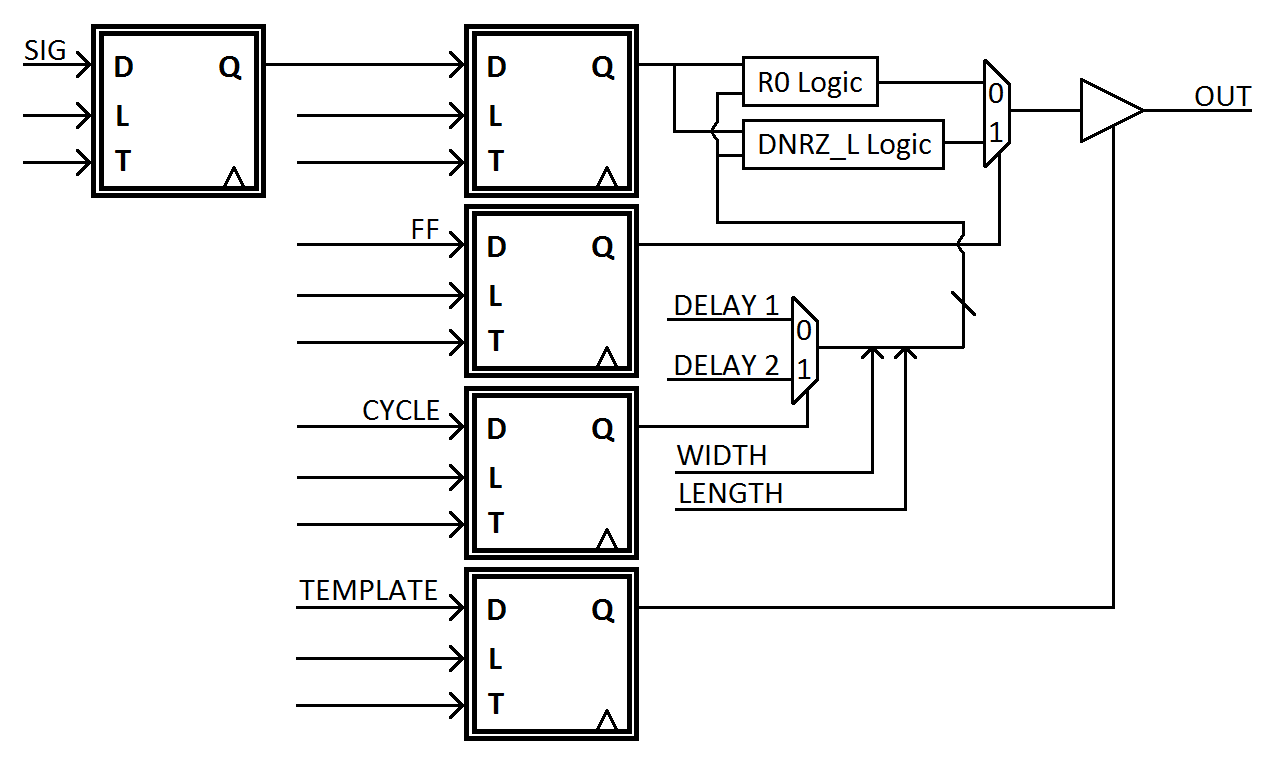
\includegraphics[width=1.0\textwidth]{verilog_schematic_per_signal.png}
\caption{Test cycle logic.}
\label{fig:test_cycle_logic}
\end{figure}

\subsection{PCB Boards}
TODO: Norm, Daniel
\newpage